\documentclass[conference,a4paper]{IEEEtran}
\usepackage[T1]{fontenc}
\usepackage[utf8]{inputenc}
\usepackage{cite,amsmath,amssymb,graphicx,booktabs,tabularx,array,xcolor,tikz,url,balance}
\usetikzlibrary{arrows.meta,positioning,fit,backgrounds,shapes.geometric,calc}
\usepackage[hidelinks]{hyperref}
\urlstyle{same}
\newcolumntype{Y}{>{\raggedright\arraybackslash}X}
\definecolor{ink}{HTML}{18334D}
\definecolor{bluewash}{HTML}{EAF2F8}
\definecolor{teal}{HTML}{147D83}
\definecolor{tealwash}{HTML}{E8F5F3}
\definecolor{amber}{HTML}{A46B13}
\definecolor{amberwash}{HTML}{FFF4DB}
\definecolor{slate}{HTML}{536579}
\tikzset{
block/.style={draw=ink!65,fill=bluewash,rounded corners=2pt,align=center,font=\sffamily\footnotesize,inner sep=6pt,line width=.65pt},
gate/.style={block,draw=amber,fill=amberwash},
data/.style={block,draw=teal,fill=tealwash},
flow/.style={-{Latex[length=2mm]},line width=.8pt,draw=ink},
softflow/.style={flow,dashed,draw=slate},
tag/.style={font=\sffamily\scriptsize\bfseries,text=ink,align=left},
edge label/.style={font=\sffamily\scriptsize,fill=white,inner sep=2pt}}
\hyphenation{Forge-Web front-end back-end work-space}
\begin{document}
\title{ForgeWeb: Architecture-First\\Full-Stack Web Application Generation}
\author{
\IEEEauthorblockN{Pratyush Manas, Rajeev Kumar, Sachin Yash Raj, Sanaa Kumari}
\IEEEauthorblockA{Department of Computer Science and Engineering\\
BMS Institute of Technology and Management, Bengaluru, India\\
1BY23CS163\quad 1BY23CS171\quad 1BY23CS192\quad 1BY23CS202}}
\maketitle

\begin{abstract}
ForgeWeb translates product descriptions into reviewed requirements and an approved architecture before coordinating source generation. The revised design retains Gemini for planning and React output and proposes a locally fine-tuned, pretrained LLaMA-based model for Python FastAPI generation. The workspace exposes files, previews, versions, and requirement links. Fourteen prior platform tests and type checking support the existing workflow, not the proposed model. Training data, checkpoint selection, and code-quality evaluation remain to be finalized. This paper separates implemented artifact management from proposed model adaptation and identifies execution-based testing as the next acceptance boundary.
\end{abstract}
\begin{IEEEkeywords}
AI-assisted development, web application generation, local language models, fine-tuning, requirement traceability.
\end{IEEEkeywords}

\section{Introduction}
Turning a customer brief into software requires decisions about screens, data, permissions, and interactions. The result must represent the requested product: a restaurant needs a booking journey rather than a renamed dashboard, and an explicit color preference must affect the rendered interface.

Recent research connects language models to requirements specification, architectural reasoning, and code generation. ReqInOne addresses requirements-document generation~\cite{ieee1}, while requirements-to-code work examines the transition toward implementation~\cite{ieee2}. Empirical SRS evaluation also makes requirements quality a research concern~\cite{ieee3}. Building an application introduces further coordination across screens, routes, and files, with opportunities for users to correct the intended design before generation.

ForgeWeb connects a prompt, an approved specification, generated artifacts, and recorded checks. The revised backend design adapts a pretrained LLaMA-based model for local code generation; it does not claim a newly pretrained foundation model. The platform's own interface remains separate from the customer's requested design. Local backend inference does not make the whole pipeline offline because planning and frontend generation still use Gemini.

\section{Problem Statement and Objectives}
Product descriptions combine features, preferences, and unstated assumptions. Generation may change a name while retaining an unsuitable layout, and an attractive preview may conceal missing server behavior. The problem is to preserve product intent while exposing enough evidence to assess the result. ForgeWeb creates an architecture file before implementation and supports revision, approval, source inspection, and version history. Its objectives are to respect explicit design choices, coordinate frontend and backend contracts, and separate artifact creation from runtime correctness.

\section{Related Work}
\subsection{Requirements and Architectural Decisions}
The requirements studies~\cite{ieee1,ieee2,ieee3} motivate making the specification inspectable before implementation. Architectural-decision generation~\cite{ieee4} and research on LLM assistance in architecture design~\cite{ieee13} address a related stage: choosing and documenting design decisions. ForgeWeb uses an architecture document as an approval boundary, without claiming to be the first system to combine requirements and code generation.

\subsection{Agents and Human Participation}
SALLMA studies architecture for LLM-based multi-agent systems~\cite{ieee5}, while SOEN-101 connects code generation to software-process roles~\cite{ieee6}. Human-in-the-loop development agents~\cite{ieee7} provide a relevant comparison for user participation. Design and refactoring frameworks~\cite{ieee18}, multi-agent code-generation studies~\cite{ieee19}, and retrieval/communication-oriented agent architectures~\cite{ieee20} broaden this setting. ForgeWeb contributes a particular workflow integration; its present task records should not be confused with independently reasoning agents.

\subsection{Local Generation and Traceability}
Research on locally deployed open-source models~\cite{ieee9} motivates evaluating the proposed local backend generator under actual hardware constraints. CodeWisp examines retrieval-guided code generation and completion~\cite{ieee10}, suggesting a future source-context mechanism. Neither establishes which checkpoint ForgeWeb should adopt.

Architecture-component extraction~\cite{ieee8}, LiSSA~\cite{ieee15}, Code Gradients~\cite{ieee16}, and security-requirement trace recovery~\cite{ieee17} address different ways to connect software artifacts. ForgeWeb instead records requirement-to-file associations during generation. Those associations aid inspection but do not establish semantic satisfaction or security enforcement.

\subsection{Validation and Research Position}
Assured LLM-based engineering~\cite{ieee11}, static-analysis-assisted review~\cite{ieee12}, and interactive code-generation evaluation~\cite{ieee21} motivate feedback beyond text generation. Accuracy/quality/performance evaluation~\cite{ieee14}, holistic evaluation~\cite{ieee22}, and a code-generation review~\cite{ieee23} support assessing several quality dimensions. Unit-test generation~\cite{ieee24} and industrial acceptance-test generation~\cite{ieee25} are relevant to future executable checks. ForgeWeb's contribution is the integration of planning, approval, generation, and project history; superiority over these approaches requires comparative experiments and is not claimed here.

\section{System Architecture}
\begin{figure*}[!t]
\centering
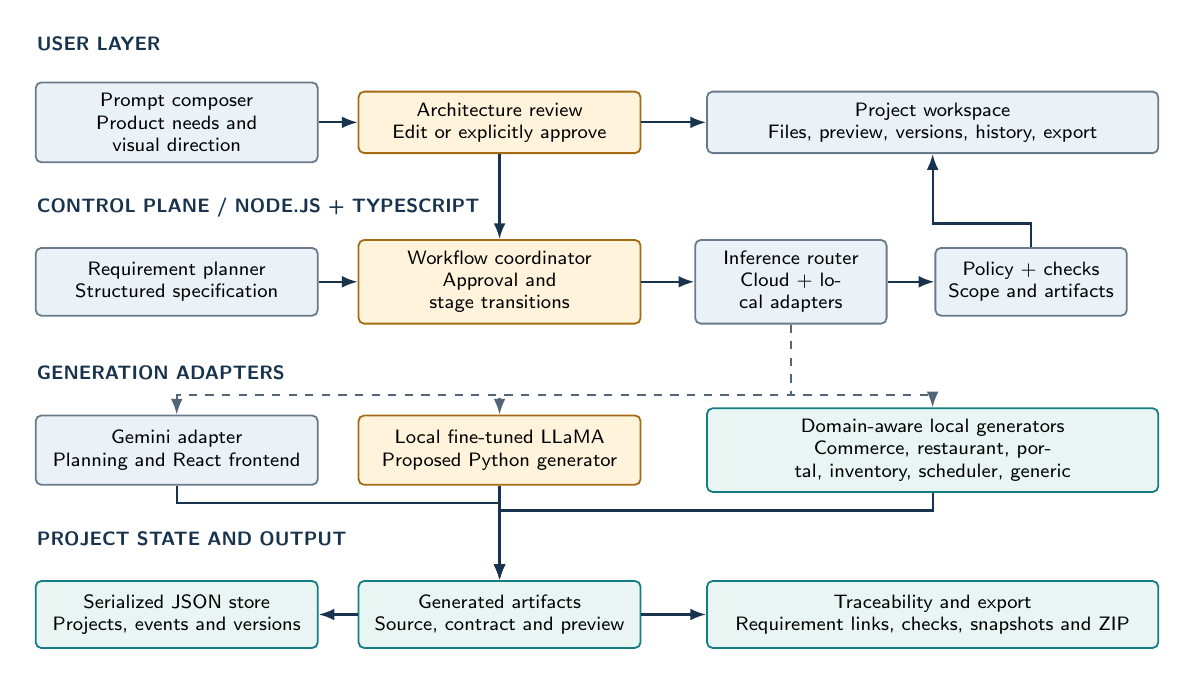
\begin{tikzpicture}[x=1cm,y=1.25cm,block/.append style={font=\sffamily\scriptsize,inner sep=4pt}]
\node[tag,anchor=west] at (0,0.45) {USER LAYER};
\node[block,text width=3.3cm,minimum height=.78cm] (prompt) at (1.9,-.35) {Prompt composer\\\scriptsize Product needs and visual direction};
\node[gate,text width=3.3cm,minimum height=.78cm] (approval) at (6,-.35) {Architecture review\\\scriptsize Edit or explicitly approve};
\node[block,text width=5.45cm,minimum height=.78cm] (workspace) at (11.5,-.35) {Project workspace\\\scriptsize Files, preview, versions, history, export};
\draw[flow] (prompt)--(approval);
\draw[flow] (approval)--(workspace);
\node[tag,anchor=west] at (0,-1.22) {CONTROL PLANE / NODE.JS + TYPESCRIPT};
\node[block,text width=3.3cm,minimum height=.86cm] (planner) at (1.9,-1.97) {Requirement planner\\\scriptsize Structured specification};
\node[gate,text width=3.3cm,minimum height=.86cm] (workflow) at (6,-1.97) {Workflow coordinator\\\scriptsize Approval and stage transitions};
\node[block,text width=2.15cm,minimum height=.86cm] (router) at (9.7,-1.97) {Inference router\\\scriptsize Cloud + local adapters};
\node[block,text width=2.15cm,minimum height=.86cm] (checks) at (12.75,-1.97) {Policy + checks\\\scriptsize Scope and artifacts};
\draw[flow] (approval.south)--(workflow.north);
\draw[flow] (planner)--(workflow);
\draw[flow] (workflow)--(router);
\draw[flow] (router)--(checks);
\draw[flow] (checks.north)--++(0,.24)-|(workspace.south);
\node[tag,anchor=west] at (0,-2.89) {GENERATION ADAPTERS};
\node[block,text width=3.3cm,minimum height=.88cm] (gemini) at (1.9,-3.68) {Gemini adapter\\\scriptsize Planning and React frontend};
\node[gate,text width=3.3cm,minimum height=.88cm] (llama) at (6,-3.68) {Local fine-tuned LLaMA\\\scriptsize Proposed Python generator};
\node[data,text width=5.45cm,minimum height=.88cm] (local) at (11.5,-3.68) {Domain-aware local generators\\\scriptsize Commerce, restaurant, portal, inventory, scheduler, generic};
\draw[softflow] (router.south)--(9.7,-3.12)-|(gemini.north);
\draw[softflow] (router.south)--(9.7,-3.12)-|(llama.north);
\draw[softflow] (router.south)--(9.7,-3.12)-|(local.north);
\node[tag,anchor=west] at (0,-4.58) {PROJECT STATE AND OUTPUT};
\node[data,text width=3.3cm,minimum height=.85cm] (store) at (1.9,-5.35) {Serialized JSON store\\\scriptsize Projects, events and versions};
\node[data,text width=3.3cm,minimum height=.85cm] (artifacts) at (6,-5.35) {Generated artifacts\\\scriptsize Source, contract and preview};
\node[data,text width=5.45cm,minimum height=.85cm] (graph) at (11.5,-5.35) {Traceability and export\\\scriptsize Requirement links, checks, snapshots and ZIP};
\draw[flow] (gemini.south)--++(0,-.18)-|(artifacts.north);
\draw[flow] (llama.south)--(artifacts.north);
\draw[flow] (local.south)--++(0,-.18)-|(artifacts.north);
\draw[flow] (artifacts)--(store);
\draw[flow] (artifacts)--(graph);
\end{tikzpicture}

\caption{Revised system architecture: the existing control plane with a proposed locally fine-tuned LLaMA backend generator. Gemini remains responsible for planning and frontend output. The trained checkpoint is not yet evaluated.}
\label{fig:architecture}
\end{figure*}
\subsection{User Layer and Control Service}
The user layer uses React and TypeScript. It contains the prompt composer, proposal review, project drawer, file viewer, preview, and version controls. A Node.js HTTP service coordinates these operations, with Vite middleware exposing the same handler during development. Workflow states distinguish planning, confirmation, generation, review, validation, and completion or failure. Figure~\ref{fig:architecture} outlines this separation.

Project state is persisted in a local JSON store. Queued writes and temporary-file replacement reduce conflicts within the local process. This arrangement supports the prototype, but is not a substitute for a transactional multi-tenant database. Database information shown in the workspace describes intended application entities; it does not prove that a database has been provisioned.

\subsection{Generation and Artifact Storage}
The proposed split pipeline uses Gemini for planning and frontend generation and a locally served, fine-tuned LLaMA-based model for backend source. A local inference adapter would receive the approved architecture, entities, routes, and API contract, then return a validated file manifest. Backend generation would no longer depend on a hosted backend-code API. The local checkpoint, model size, hardware, and serving configuration are not yet fixed; no latency or privacy improvement is claimed without measurement.

Local generators cover selected commerce, restaurant, portal, inventory, scheduling, and generic-site cases. They provide a bounded fallback rather than unlimited design originality. Generator mode and failure messages remain attached to the result. Stored artifacts include source, a shared contract, documentation, preview HTML, and file digests. Snapshots support inspection, restoration, and ZIP export.

\subsection{Proposed Model Adaptation}
Training would pair architecture and API specifications with reviewed Python implementations. Data must be license-compatible, stripped of secrets, deduplicated, and split by project to reduce train--test leakage. A pretrained LLaMA-based checkpoint would be fine-tuned on these pairs and served locally after evaluation. The untouched base model and adapted model should be compared on held-out builds, API behavior, and authorization tests. Checkpoint identity, dataset provenance, training settings, and hardware must be recorded before reporting results.

\section{Methodology}
\subsection{Planning and Approval}
The planner turns a validated prompt into a proposed specification and \texttt{ARCHITECTURE.md}. Explicit names and visual preferences should survive normalization. The user can edit the request or confirm the proposal; implementation begins only after confirmation. This boundary checks agreement about scope, not the correctness of later code. Figure~\ref{fig:flow} shows the sequence and failure branch.

\begin{figure}[!ht]
\centering
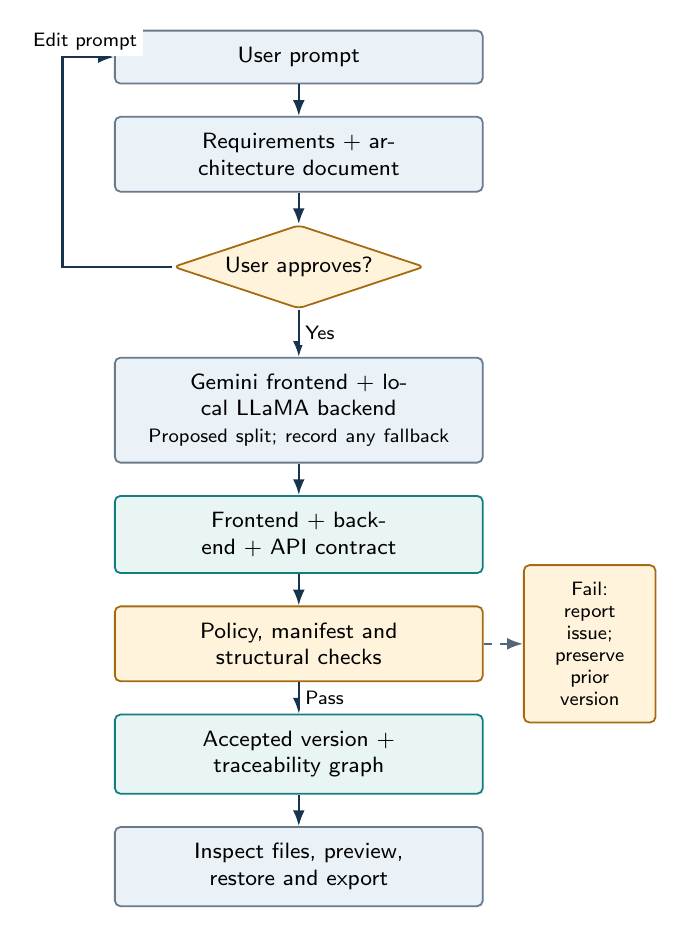
\begin{tikzpicture}[node distance=4mm]
\node[block,text width=4.25cm] (prompt) {User prompt};
\node[block,text width=4.25cm,below=of prompt] (plan) {Requirements + architecture document};
\node[gate,diamond,aspect=3,inner sep=2pt,below=of plan] (gate) {User approves?};
\node[block,text width=4.25cm,below=6mm of gate] (gen) {Gemini frontend + local LLaMA backend\\\scriptsize Proposed split; record any fallback};
\node[data,text width=4.25cm,below=of gen] (files) {Frontend + backend + API contract};
\node[gate,text width=4.25cm,below=of files] (check) {Policy, manifest and structural checks};
\node[data,text width=4.25cm,below=of check] (save) {Accepted version + traceability graph};
\node[block,text width=4.25cm,below=of save] (preview) {Inspect files, preview, restore and export};
\draw[flow] (prompt)--(plan);
\draw[flow] (plan)--(gate);
\draw[flow] (gate)--node[edge label,right]{Yes}(gen);
\draw[flow] (gate.west)--(-3,0 |- gate.west) |- node[edge label,pos=.72,above]{Edit prompt} (prompt.west);
\draw[flow] (gen)--(files);
\draw[flow] (files)--(check);
\draw[flow] (check)--node[edge label,right]{Pass}(save);
\draw[flow] (save)--(preview);
\node[gate,text width=1.25cm,font=\sffamily\scriptsize,right=5mm of check] (fail) {Fail:\\report issue;\\preserve prior version};
\draw[softflow] (check.east)--(fail.west);
\end{tikzpicture}

\caption{Revised data flow with proposed local-model backend generation. A recorded template fallback is distinct from model inference.}
\label{fig:flow}
\end{figure}

\subsection{Frontend and Backend Coordination}
The approved specification guides React source, styles, FastAPI routes, schemas, access-control files, and supporting tests. A shared JSON contract expresses the intended route and data agreement. Figure~\ref{fig:structure} separates these files from the preview path. Contract presence reduces ambiguity but cannot establish that implementations agree: a booking form and its endpoint can still interpret dates or identifiers differently.

\begin{figure}[!ht]
\centering
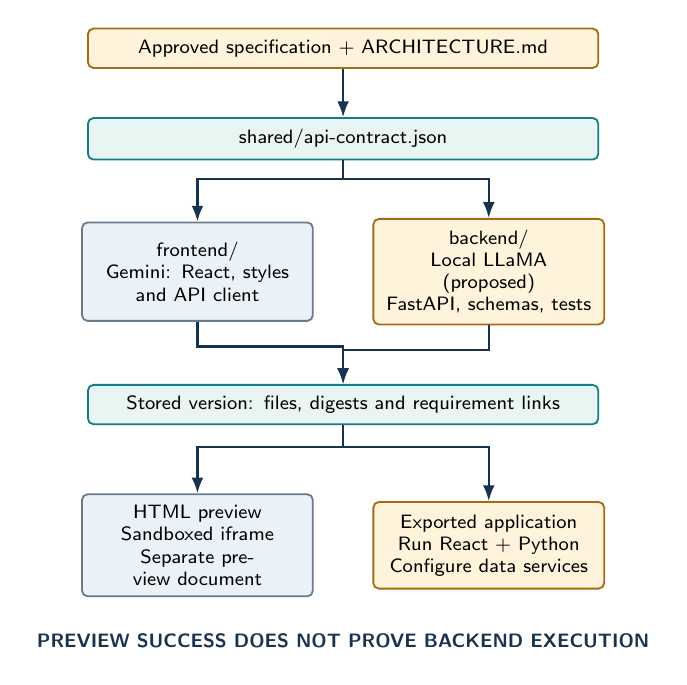
\begin{tikzpicture}[x=1cm,y=1.25cm,block/.append style={font=\sffamily\scriptsize,inner sep=4pt}]
\node[gate,text width=6.2cm] (spec) at (0,0) {Approved specification + ARCHITECTURE.md};
\node[data,text width=6.2cm] (contract) at (0,-.92) {shared/api-contract.json};
\node[block,text width=2.65cm,minimum height=1.25cm] (front) at (-1.85,-2.27) {frontend/\\\scriptsize Gemini: React, styles\\and API client};
\node[gate,text width=2.65cm,minimum height=1.25cm] (back) at (1.85,-2.27) {backend/\\\scriptsize Local LLaMA (proposed)\\FastAPI, schemas, tests};
\draw[flow] (spec)--(contract);
\draw[flow] (contract.south)--++(0,-.19)-|(front.north);
\draw[flow] (contract.south)--++(0,-.19)-|(back.north);
\node[data,text width=6.2cm] (version) at (0,-3.62) {Stored version: files, digests and requirement links};
\draw[flow] (front.south)--++(0,-.25)-|(version.north);
\draw[flow] (back.south)--++(0,-.25)-|(version.north);
\node[block,text width=2.65cm,minimum height=1.1cm] (prev) at (-1.85,-5.05) {HTML preview\\\scriptsize Sandboxed iframe\\Separate preview document};
\node[gate,text width=2.65cm,minimum height=1.1cm] (run) at (1.85,-5.05) {Exported application\\\scriptsize Run React + Python\\Configure data services};
\draw[flow] (version.south)--++(0,-.22)-|(prev.north);
\draw[flow] (version.south)--++(0,-.22)-|(run.north);
\node[tag,align=center] at (0,-6.02) {PREVIEW SUCCESS DOES NOT PROVE BACKEND EXECUTION};
\end{tikzpicture}

\caption{Generated artifacts under the proposed split: Gemini frontend and locally fine-tuned LLaMA backend. Preview and application execution remain separate.}
\label{fig:structure}
\end{figure}

The embedded preview runs stored HTML in an iframe with script and form permissions. It does not start the generated Python service. Local preview interactions must therefore be distinguished from verified frontend-to-backend requests. Running the exported application requires its dependencies and data services to be configured.

\subsection{Review and Traceability}
Planning, implementation, review, and validation records describe objectives, allowed paths, and acceptance criteria. Project policy draws on the supplied Karpathy-derived engineering guidance and gstack workflow material: clarify assumptions, prefer a sufficient solution, limit changes to scope, and inspect evidence. These engineering repositories are not counted as research publications.

The current checks examine paths, manifests, expected artifacts, requirement mappings, and provenance. The internal graph links projects, requirements, tasks, files, and checks. A requirement-to-file edge records an association, not proof that a feature works. Similarly, the graph is not an externally parsed call graph from Code Review Graph. Stronger acceptance would combine the current structural checks with clean builds, API requests, and browser interaction tests against the generated application.

\section{Evaluation and Discussion}
The earlier platform evaluation passed fourteen top-level tests and TypeScript checking. Table~\ref{tab:results} reports that baseline, not a rerun of a local-model integration. Temporary stores and deterministic or injected responses exercise orchestration; no fine-tuned checkpoint was tested. Local-model accuracy, runtime, and resource use remain unmeasured.

\begin{table}[!ht]
\caption{Prior Platform Checks (Not Local-Model Results)}
\label{tab:results}
\centering\footnotesize
\begin{tabularx}{\columnwidth}{@{}Ycc@{}}
\toprule
Test group & Cases & Result\\
\midrule
HTTP and approval lifecycle & 2 & Passed\\
Domain and visual instructions & 4 & Passed\\
Provider fixture and selection & 2 & Passed\\
Plan normalization & 1 & Passed\\
Workspace, versions, compatibility & 3 & Passed\\
Prompt and path rejection & 2 & Passed\\
\midrule
Total & 14 & Passed\\
Platform type checking & --- & Passed\\
\bottomrule
\end{tabularx}
\end{table}

Approval checks enforce confirmation before implementation. Domain checks examine product-specific output and explicit colors, but not perceived uniqueness. Workspace checks cover snapshots, restoration, persistence, export, and safe failure. Provider fixtures verify plan and manifest handling, not live availability.

The results support the orchestration and artifact-management design. They do not establish secure deployment, payment correctness, or successful execution of every generated interaction. A useful next experiment would compare direct generation with architecture-first generation on the same prompts and provider settings. Measurements should include requirement-level task success, contract agreement, clean-build success, visual adherence, latency, and cost. Such comparative measurements have not been conducted here.

\section{Limitations and Future Work}
Source checks can miss broken handlers, incorrect permissions, and mismatched payloads. Fallback designs remain limited, model responses vary, and local persistence is unsuitable for production-scale tenancy.

The immediate priority is selecting, fine-tuning, and evaluating the local LLaMA-based checkpoint, then connecting its manifest output to the workflow. Isolated execution, persistent application data, and browser tests remain necessary. Training does not itself establish code correctness or security, and human assessment must verify visual requirements.

\section{Conclusion}
ForgeWeb makes planning and approval explicit before source generation. The revised design combines Gemini-assisted frontend generation with a proposed locally fine-tuned LLaMA backend model. Existing checks support the surrounding workflow, not the untested checkpoint. Training evidence and executed application tests are needed before assessing the revised pipeline's effectiveness.

\bibliographystyle{IEEEtran}
\bibliography{references-ieee}
\end{document}
